\documentclass{ximera}

%\addPrintStyle{..}

\begin{document}
	\author{Bart Lambregs}
	\xmtitle{Eenparige versnelde rechtlijnige beweging}{}
    \xmsource\xmuitleg



De ééndimensionale beweging met een constante  versnelling wordt de \textit{eenparig veranderlijke rechtlijnige beweging} genoemd (EVRB). 
Eenparig betekent gelijkmatig; bij een constante versnelling is de \textit{verandering} van de snelheid steeds gelijk.
De grafiek van $a(t)=a$ is een constante met $a$ een reëel getal is.
Ook voor deze beweging kan je de plaatsfunctie en snelheidsfunctie bepalen en zo het verloop van de plaats en snelheid in functie van de tijd kennen. 


De versnelling is de afgeleide van de snelheid. 
Voor een constante versnelling is de snelheid in functie van de tijd een lineaire functie (in de tijd).


\begin{remark}
	Strikt genomen wordt hier iets over het hoofd gezien. 
	A priori zou het immers kunnen dat er nog andere functies dan lineaire functies zijn waarvoor de afgeleide een constante functie is. 
	Dat is echter niet het geval. 
	Het bewijs hiervan zie je later dit jaar in het vak wiskunde. 
	Je bewijst dat alle mogelijke functies die in aanmerking komen slechts op een constante na aan elkaar gelijk zijn. 
\end{remark}

Uit het snelheidsverloop kan je de plaats afleiden. 
De snelheid is de afgeleide van de plaatsfunctie. 
Voor een lineaire snelheidsfunctie is de positie bijgevolg een kwadratische functie (in de tijd). 
De afgeleide van een kwadratische functie is immers een lineaire functie.\footnote{Hier geldt een gelijkaardige opmerking.}
	
Dat de positie in functie van de tijd een tweedegraadsveeltermfunctie is, geeft in symbolen: 

% \footnote{we gebruiken de constanten $p$, $q$ en $r$ i.p.v. $a$, $b$ en $c$ om verwarring met de betekenis van $a$ te voorkomen.}

\[
x(t)=pt^2+qt+r
\]

De constanten $p$, $q$ en $r$ is deze formule hebben een fysische betekenis. 
De snelheid is de afgeleide van deze plaatsfunctie en de versnelling komt overeen met de tweede afgeleide. Dit levert: 

% GEWIJZIGTD NAAR X(t); kan weggelaten worden 
\[
v(t) =\frac{dx(t)}{dt}=2pt+q
\]

\[
a(t) =\frac{d^2x(t)}{dt^2}=2p
\]

Voor de EVRB is de versnelling constant en bijgevolg volgt uit de laatste regel dat $a(t)=a=2p\Leftrightarrow p=\frac{a}{2}$. 

Noteer met $v_0=v(0)$ de snelheid op tijdstip $t=0$. In de eerste vergelijking $t=0$ invullen levert dan $q=v_0$. De constante $q$ stelt de beginsnelheid voor. 

Noteer met $x_0=x(0)$ de positie op tijdstip $t=0$. In de plaatsfunctie $t=0$ invullen levert dan $r=x_0$. De constante $r$ stelt dus de beginpositie voor.


\begin{theorem}
De plaatsfunctie $x(t)$ en de snelheidsfunctie $v(t)$ van een EVRB met versnelling $a$ worden gegeven door:
\[
\begin{array}{rcl}
x(t)&=&x_0+v_0t+\frac{1}{2}at^2\\
v(t)&=&v_0+at
\end{array}
\]
Hierin is $x_0$ de \textit{beginpositie} en $v_0$ de \textit{beginsnelheid}. Ze worden bepaald door de \textit{beginvoorwaarden} of \textit{randvoorwaarden}.
\end{theorem}	

Indien de beschrijving van de beweging niet op $t=0$ start maar op een gegeven tijdstip $t_0$, dan wordt in de beschrijving $t$ vervangen door $\Delta t= t-t_0$, de verstreken tijd vanaf het begintijdstip $t_0$. De plaatsfunctie en zijn afgeleide worden dan een klein beetje ingewikkelder:

\[
x(t) = x_0+v_0(t-t_0)+\frac{1}{2}a(t-t_0)^2
\]

\[
v(t) = v_0+a(t-t_0)
\]

Met de functies kan je de volgende formule voor de gemiddelde snelheid van een EVRB aantonen:

%\footnote{Het formuletje is handig te gebruiken in veel vraagstukken door gebruik te maken van $\Delta x=\overline{v}\Delta t$.} 

\[
\overline{v}=\frac{v_0+v}{2}
\]
	
\begin{exercise}
Bewijs bovenstaande formule. 

\begin{hint}
Gebruik de definitie voor gemiddelde snelheid en bereken de verplaatsing met de plaatsfunctie voor de EVBR. 
\end{hint}

\begin{oplossing}
	\[
	\overline{v}=\frac{\Delta x}{\Delta t}=\frac{x-x_0}{t-t_0} = \frac{v_0(t-t_0)+\frac{1}{2}a(t-t_0)^2}{(t-t_0)} = \frac{2v_0+a(t-t_0)}{2} = \frac{2v_0 + v - v_0}{2} = \frac{v_0+v}{2}.
	\]
		
	bij een EVRB kan je dus het rekenkundig gemiddelde gebruiken om de gemiddelde snelheid te berekenen. 
	In onderstaande figuur is \(\overline{v}\) grafisch weergegeven als het midden van de lineaire snelheidsfunctie. 

	\begin{image}
		\begin{tikzpicture}
			% axes
			\draw[->] (0,0) -- (4,0) node[right] {tijd};
			\draw[->] (0,0) -- (0,2.5) node[above] {snelheid};
			% lines

			\coordinate (X) at (0,1);
			\coordinate (Y) at (3,2);
            \coordinate (M) at ($ (X)!0.5!(Y) $);

			\fill (X) circle (2pt) node[left] {$v_0$};
			\fill (Y) circle (2pt) node[above] {$v(t)$};
			\fill (M) circle (2pt) node[above, red, thick] {$\overline{v}$};
			% \fill (M) circle (2pt) node[above] {$\overline{v} = \frac{v_0 + v}{2}$};

			\draw (X) -- (Y);  

			\draw[dashed] (Y) -- (3, 0) node[below]{\(t\)};
		\end{tikzpicture}
	\end{image}

\end{oplossing}

% TODO; DIT IS NIET HELEMAAL CORRECT; ZE KENNEN DIT ALS MIDDEN VAN EEN LIJNSTUK BEREKENEN. 
	
\end{exercise}






\begin{image}[0.5 \textwidth]
	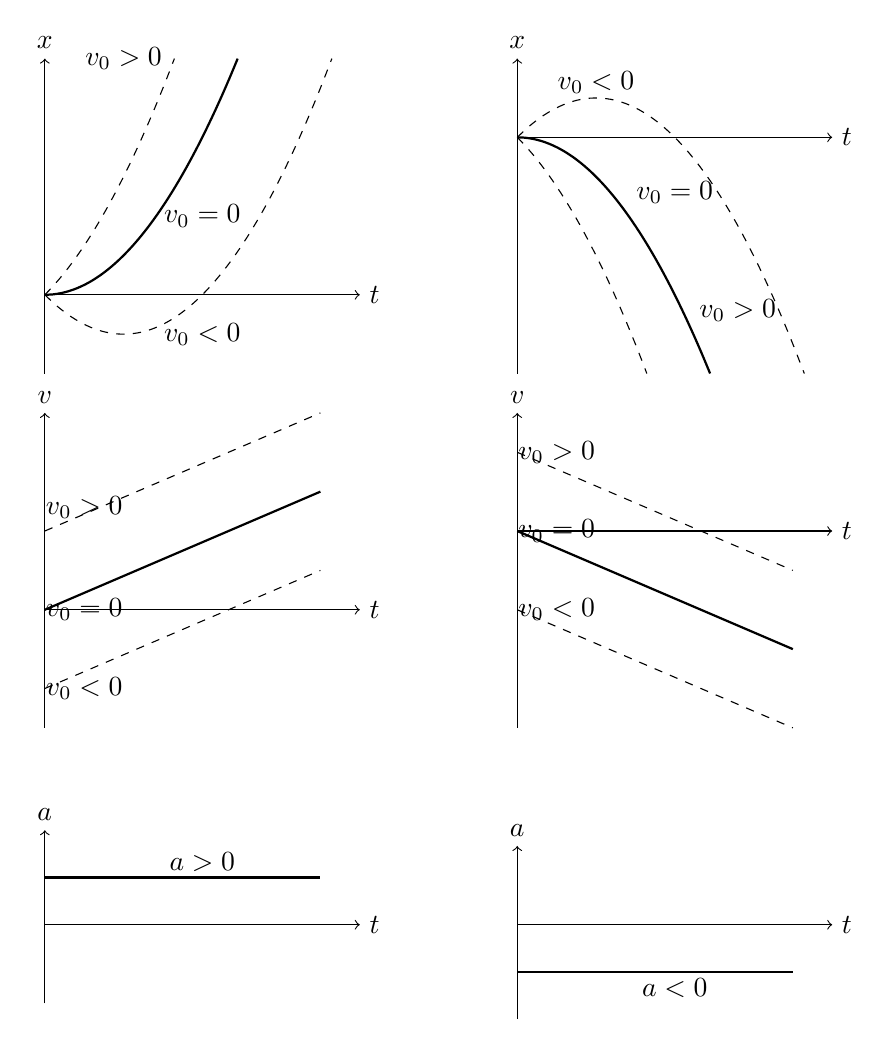
\begin{tikzpicture}
		\begin{scope}[shift={(0,8)}]
			% set maximum y value
			\def\ymax{3}
		
			% axes
			\draw[->] (0,0) -- (4,0) node[right] {$t$};
			\draw[->] (0,-1) -- (0, \ymax ) node[above] {$x$};
		
			% case v0 = 1
			\pgfmathsetmacro{\tmaxA}{-1 + sqrt(1^2 + 2*\ymax)}
			\draw[dashed, domain=0:\tmaxA, smooth] plot (\x,{0.5*\x*\x + 1*\x});
		
			% case v0 = 0
			\pgfmathsetmacro{\tmaxB}{sqrt(2*\ymax)}
			\draw[thick, domain=0:\tmaxB, smooth] plot (\x,{0.5*\x*\x});
		
			% case v0 = -1
			\pgfmathsetmacro{\tmaxC}{1 + sqrt((-1)^2 + 2*\ymax)}
			\draw[dashed, domain=0:\tmaxC, smooth] plot (\x,{0.5*\x*\x - 1*\x});
		
			% labels
			\node at (1.0,3.0) {$v_0>0$};
			\node at (2.0,1.0) {$v_0=0$};
			\node at (2.0,-0.5) {$v_0<0$};
		\end{scope}
	
		\begin{scope}[shift={(6,10)}]
			% set minimum y value (negative cutoff)
			\def\ymin{-3}
		
			% axes
			\draw[->] (0,0) -- (4,0) node[right] {$t$};
			\draw[->] (0,\ymin) -- (0,1) node[above] {$x$};
		
			% case v0 = -1
			\pgfmathsetmacro{\tmaxA}{-1 + sqrt((-1)^2 - 2*\ymin)} % = v0 + sqrt(v0^2 - 2*ymin)
			\draw[dashed, domain=0:\tmaxA, smooth] plot (\x,{-0.5*\x*\x - 1*\x});
		
			% case v0 = 0
			\pgfmathsetmacro{\tmaxB}{sqrt(-2*\ymin)}
			\draw[thick, domain=0:\tmaxB, smooth] plot (\x,{-0.5*\x*\x});
		
			% case v0 = 1
			\pgfmathsetmacro{\tmaxC}{1 + sqrt(1 - 2*\ymin)}
			\draw[dashed, domain=0:\tmaxC, smooth] plot (\x,{-0.5*\x*\x + 1*\x});
		
			% labels
			\node at (1.0,0.7) {$v_0<0$};
			\node at (2.0,-0.7) {$v_0=0$};
			\node at (2.8,-2.2) {$v_0>0$};
		\end{scope}
	
		% ====== Velocity vs Time (a > 0) ======
		\begin{scope}[shift={(0,4)}]
			% axes
			\draw[->] (0,0) -- (4,0) node[right] {$t$};
			\draw[->] (0,-1.5) -- (0,2.5) node[above] {$v$};
			% lines
			\draw[dashed] (0,1) -- (3.5,2.5);
			\draw[thick]  (0,0) -- (3.5,1.5);
			\draw[dashed] (0,-1) -- (3.5,0.5);
			% labels
			\node at (0.5,1.3) {$v_0>0$};
			\node at (0.5,0.0) {$v_0=0$};
			\node at (0.5,-1.0) {$v_0<0$};
		\end{scope}
			
		% ====== Velocity vs Time (a < 0) ======
		\begin{scope}[shift={(6,5)}]
				% axes
				\draw[->] (0,0) -- (4,0) node[right] {$t$};
				\draw[->] (0,-2.5) -- (0,1.5) node[above] {$v$};
				% lines
				\draw[dashed] (0,1) -- (3.5,-0.5);
				\draw[thick]  (0,0) -- (3.5,-1.5);
				\draw[dashed] (0,-1) -- (3.5,-2.5);
				% labels
				\node at (0.5,1.0) {$v_0>0$};
				\node at (0.5,0.0) {$v_0=0$};
				\node at (0.5,-1.0) {$v_0<0$};
		\end{scope}
	
		% ====== Acceleration vs Time (a > 0) ======
		\begin{scope}[shift={(0,0)}]
			% axes
			\draw[->] (0,0) -- (4,0) node[right] {$t$};
			\draw[->] (0,-1) -- (0,1.2) node[above] {$a$};
			% constant acceleration
			\draw[thick] (0,0.6) -- (3.5,0.6);
			% label
			\node at (2,0.8) {$a>0$};
		\end{scope}
		
		% ====== Acceleration vs Time (a < 0) ======
		\begin{scope}[shift={(6,0)}]
			% axes
			\draw[->] (0,0) -- (4,0) node[right] {$t$};
			\draw[->] (0,-1.2) -- (0,1) node[above] {$a$};
			% constant acceleration
			\draw[thick] (0,-0.6) -- (3.5,-0.6);
			% label
			\node at (2,-0.8) {$a<0$};
		\end{scope}
		
	\end{tikzpicture}
	\end{image}
	\captionof{figure}{Grafieken van de EVRB}
	
	


\begin{exercise}

Een auto die $\SI{60}{km/h}$ rijdt, raakt een boom; de voorkant van de auto wordt in elkaar gedrukt en de bestuurder komt na $\SI{70}{cm}$ tot stilstand. Welke gemiddelde vertraging onderging de bestuurder tijdens de botsing? Druk je antwoord uit in $g$, waarbij $g=\SI{9,81}{m/s^2}$.
% \textit{Gegeven}  $v_0=\SI{16,7}{m/s}$%%%\newline$x=\SI{0,70}{m}$
% \textit{Gevraagd} $a$
% \textit{Oplossing} 
\begin{oplossing} 
Om de (constante) vertraging te vinden, hebben we de snelheidsverandering en de benodigde tijd nodig. De verandering in snelheid kennen we; de eindsnelheid van de auto moet nul worden maar de duur is niet onmiddellijk gegeven. Omdat de eindsnelheid nul is, kunnen we wel uit de snelheidsvergelijking van een eenparig veranderlijke beweging een \emph{uitdrukking} vinden voor die tijd die we vervolgens kunnen substitueren in de plaatsvergelijking. De enige onbekende is dan de gezochte versnelling.\footnote{M.b.v. de formule $\overline{v}=\frac{v_0+v}{2}$ voor de gemiddelde snelheid en de definitie voor de gemiddelde snelheid $\overline{v}=\frac{\Delta x}{\Delta t}$ is het antwoord sneller te vinden. Ga maar na \ldots}
%%%\newline
%%%\newline
Uit $v(t)=0$ of $0=v_0+at$ halen we een uitdrukking voor de tijd die nodig is om tot stilstand te komen:
\begin{align*}
t&=-\frac{v_0}{a}
\end{align*}
Substitutie van deze tijd in de plaatsfunctie levert:
\begin{align*}
x&=v_0t+\frac{1}{2}at^2\\
&=v_0\left(-\frac{v_0}{a}\right)+\frac{1}{2}a\left(-\frac{v_0}{a}\right)^2\\
%&=&-\frac{v_0^2}{a}+\frac{v_0^2}{2a}\\
&=-\frac{v_0^2}{2a}\\
\end{align*}
De versnelling is dan gelijk aan:
\begin{align*}
a&=-\frac{v_0^2}{2x}
\end{align*}
Invullen van de gegevens levert $a=\SI{-198}{m/s^2}$, wat gelijk is aan $20g$.
\end{oplossing}
\end{exercise}



	
	
\end{document}
